\documentclass[a4paper]{book}
\usepackage{parskip}
\usepackage[top=2.0cm,bottom=2.0cm,left=1.5cm,right=1.5cm]{geometry}
\usepackage{amsmath}
\usepackage{amsfonts}
\usepackage{graphicx}
\def\cX {\mathcal{X}}
\def \xl {x^{(l)}}
\def \bxl{\mathbf{x}^{(l)}}
\def \xil {x^{(l)}_i}
\def\x{\mathbf{x}}
\def\bx{\mathbf{x}}
\def \cL {\mathcal{L}}
\def \bw {\mathbf{w}}
\def \w {mathbf{w}}
\def \sumln {\sum_{l=1}^N}
\def \r {\mathbf{r}}
\def \brl {\mathbb{r}^{(l)}}
\def \bmu {\boldsymbol\mu}
\def \bSig {\boldsymbol\Sigma}
\def \bPhi {\boldsymbol\Phi}
\def \byl {\mathbf{y}^{(l)}}
\def \by{\mathbf{y}}
\def \yil {y^{(l)}_i}
\def \yl{y^{(l)}}
\def \cN {\mathcal{N}}
\def \rl {r^{(l)}}
\def \bD {\mathbf{D}}
\def \bm {\mathbf{m}}
\def \cG {\mathcal{G}}
\def \bz {\mathbf{z}}
\def \zl {z^{(l)}}
\def \bzl{\mathbf{z}^{(l)}}
\def \bS {\mathbf{S}}
\def \cQ {\mathcal{Q}}
\def \bm {\mathbf{m}}
\def \bW{\mathbf{W}}
\def \cT{\mathcal{T}}
\def \cV{\mathcal{V}}
\def \bA{\mathbf{A}}
\def \bB{\mathbf{B}}
\def \bC{\mathbf{C}}
\def \bR{\mathbf{R}}
\def \ba{\mathbf{a}}
\def \brl{\mathbf{r}^{(l)}}
\def \bv{\mathbf{v}}
\def \bh{\mathbf{h}}
\title{Machine Learning}
\author{LI Tao}
\begin{document}
\maketitle
\chapter{Bayesian Decision Theory}
\begin{description}
\item[Bernoulli]: $P(X) = p_0^X(1-p_0)^{1-X}$, $p_0$ is the param.
\item Estimation of $p_0$ form $\cX = \{x^{(l)}\}^N_{l=1}$:\\ $\hat{p_0} =
\frac{\mbox{\#heads}}{\mbox{\#tosses}} = \frac{\sum^N_{l=1}x^{(l)}}{N}$
\item Predict outcome = head if $P_0 > 1/2$, tail otherwise.
\item [Baye's Rule]:\\ $\mbox{Posterior}P(C|\x) = \frac{\mbox{likelihood}\times
\mbox{prior}}{\mbox{evidence}} = \frac{p(\x|C)P(C)}{p(\x)}$
\item Baye for $K>2$ classes: \\
$P(C_i|\x) =  \frac{p(\x|C_i)P(C_i)}{\sum^K_{k=1}p(\x|C_k)P(C_k)}$
\item Optimal decision: Choose $C_i$ if $P(C_i|\x) = \max_k(C_k|\x)$
\item [Losses and Risks]: \\
$R(\alpha_i|\x) = \sum^K_{k=1} \lambda_{ik}P(C_k|\x) $,\\
$\alpha_i$ the action assigned to class 
$C_i$, $\lambda_{ik}$ loss for $\alpha_i$ if $C_k$
\item Optimal:$\alpha_i$ if $R(\alpha_i|\x) = \min_k R(\alpha_k|\x) $
\item [0-1 loss]: $R(\alpha_i|\x) = \sum_{k=1}^K\lambda_{ik}P(C_k|\x) =
    1-P(C_i|\x)$,\\$\lambda_{ik} = 1$ if $i\neq k$, $0$ otherwise
\item [Reject Option]: Loss: \[ \lambda_{ik} = \begin{cases} 
    1  &\mbox{if } i = k   \\
    \lambda & \mbox{if } i = K+1 \\
    0 & \mbox{otherwise } \end{cases}\]
$\lambda$ is the loss for choosing reject.
\item Expected risk:\[R(\alpha_i|\x) = 
\begin{cases}
    \sum_{k=1}^K\lambda P(C_k|\x) = \lambda  & \mbox{if } i = K+1\\
    \sum_{k\neq 1}P(C_k|\x) = 1 - P(C_i|\x)  & \mbox{if } i \in {1,\dots,K}
\end{cases}
\]
\item Optimal Decision: choose $C_i$ if \\$R(\alpha_i|x) = \min_{1\leq k\leq
K}R(\alpha_i|\x) < R(\alpha_{K+1} | \x)$, \\Reject otherwise.
\item [Discriminant Functions]: choose $C_i$ if $g_i(\x) = \max_k g_k(x)$
\item $g_i(\x) = -R(\alpha_i|x) = P(C_i|\x) = p(\x|C_i)P(C_i)$
\item Two class may define single discriminant functions: $g(\x) = g_1(\x) -
g_2(\x)$, choose $C_i$ if it greater than zero.
\item [Decision Regions] $\mathcal{R}_i = \{\x|g_i(\x) = \max_k g_k(\x)\}$
\item[Bayesian Network] joint:\\ $P(X_1,\dots, X_d) = \prod_{i=1}^d P(X_i|parents(X_i))$
\end{description}

\chapter{Parameter Estimation}
\begin{description}
\item[Setting] Assume data follow a distribution model.$\mathcal{X}=\{\x^{(l)}\}$, 
$\x^{l}\sim p(\x)$, Assume some
parametric form for $p(\x|\theta)$, $\theta$ is estimated using $\mathcal{X}$
\item[Param Approach to classification] In Baye's rule for classification,
$p(\x|C_i) \mbox{(likelihood) and } P(C_i)$ (prior) need to be estimated from the sample 
$\mathcal{X}$
\item[MLE] seeks to find $\theta$ that makes sampling from $p(\x|\theta)$ as
likely as possible
\item likelihood:\\$L(\theta|\mathcal{X}) \equiv p(\mathcal{X}|\theta) =
\prod^N_{l=1}p(\x^{(l)}|\theta)$
\item log likelihood: $\mathcal{L} \equiv \log L(\theta|X) = \sum^N_{l=1}\log
p(\x^{(l)}|\theta)$
    \item Max Likelihood estimate: $\hat{\theta} =
    arg\max_{\theta}\mathcal{L}(\theta|\mathcal{X})$
\item[Bernoulli] $x \in\{0, 1\}, P(x=1)$ for $p(C_1)$,\\ $P(x|p_0) =
p_0^x(1-p_0)^{1-x}$
\item[] Log Likelihood:\\ $\mathcal{L}(p_0|\cX) = \sum_{l=1}^N[x^{(l)}\log
        p_0+(1-x^{(l)})\log(1-p_0)]$
    \item[] ML estimation: $\hat{p_0} = \frac{1}{N}\sum_{l=1}^N x^{(l)}$
\item[Multinomial]Ran Var. $\x$ with $K\geq 2$ possible value
\item Indicator var: $x_i = 1 \mbox{ if outcome is state }i \mbox{, } 0 \mbox{
if not}$
\item $P(\x|\theta) = P(X_1,\dots, x_K|p_1,\dots, p_K) =
    \prod^K_{i=1}p_i^{x_i}$, $\sum_{i=1}^K p_i = 1$
\item[] Log likelihood: $\cL (p_0|\cX) = \sum_l^N\sum_{i=1}^K x_i^{(l)} \log p_i$
\item[] ML estimate: $\hat{p_i} = \frac{1}{N}\sumln \xil$
\item[Normal] pdf: $p(x|\mu, \sigma ) =
    \frac{1}{\sqrt{2\pi\sigma^2}}\exp[-\frac{(x-\mu)^2}{2\sigma^2}]$
\item[] $\cL(\mu, \sigma|\cX) = -\frac{N}{2}\log(2\pi) - N\log\sigma -
    \frac{1}{2\sigma^2}\sumln(\xl - \mu)^2$
\item ML Estimates: $\hat{\mu} = \frac{1}{N}\sumln \xl$\\
    $\hat{\sigma^2} = \frac{1}{N}\sumln (\xl - \hat{\mu})^2$
\item[Multivariable Normal] $\mathcal{N}(\bmu,\bSig)$, $\bmu$ mean vec, $\bSig$
    covariance matrix
\item[] $p(\x|\bmu, \bSig) = \frac{1}{(2\pi)^{d/2}|\bSig|^{1/2}}
    \exp[-\frac{1}{2}(\x -\bmu)^T\bSig^{-1}(\x - \bmu)]$
\item $\cL (\bmu,\bSig|\cX) = \frac{Nd}{2}\log(2\pi) - \frac{N}{2}\log|\bSig|
    -\frac{1}{2}\sumln(\bxl - \bmu)^T\bSig^{-1}(\bxl - \bmu)$
\item[] ML estimates: $\hat{\bmu} = \frac{1}{N}\sumln \bxl$, \\
    $\hat{\bSig} = \frac{1}{N}\sumln(\bxl - \hat{\bmu})(\bxl - \hat{\bmu})^T$
\item[Bias and Variance] Bias: $b_\theta(d) = E[d] - \theta$
    \\Variance: $E[d-E[d]^2]$(d is estimator of param $\theta$)
\item[] Mean Squared error: \\
    $r(d,\theta) = E[(d-\theta)^2]= \mbox{bias}^2 + \mbox{variance}^2$
\item[Bayesian Estimation] Treat $\theta$ as a Ran Var. Prior $p(\theta)$
\item[] Posterior: \\
    $p(\theta|\cX) = \frac{p(\cX|\theta)p(\theta)}{p(\cX)} =
    \frac{p(\cX|\theta)p(\theta)}{ \int p(\cX|\theta')p(\theta')d\theta'}$
\item[] Estimation of density at $x$: \\
    $p(x|\cX) = \int p(x|\theta)p(\theta|\cX)d\theta$
\item[] Regression $y = g(x|\theta)$:
    $ y = \int g(x|\theta)p(\theta|\cX)d\theta $
\item[Computational Considerations] 
\item[] Max a posteriori (MAP): $\theta_{MAP}=arg\max_{\theta}p(\theta|\cX)$,\\
    $p(x|\cX) \approx p(x|\theta_{MAP)}$, $y\approx y_{MAP} =
    g(x|\theta_{MAP}$)

    ML estimation: $\theta_{ML} = arg \max_{\theta} p(\theta|\cX)$

    Bayes' estimation -- expectation w.r.t.\ posterior density:
    \[ \theta_{Bayes} = E[\theta|\cX] = \int \theta p(\theta|\cX)d\theta\]
\item[] Example: Bayesian estimation with known $\mu$, $\sigma$ and $\sigma_0$\\
        $x^{(l)} \sim \mathcal{N}(\theta, \sigma_0^2)$, 
        $\theta  \sim \mathcal{N}(\mu, \sigma^2)$\\
         MLE: $\theta_{ML} = \frac{1}{N}\sumln\x^{(l)}=m$ \\
         $\theta_{Map} = \theta_{Bayes}  =E(\theta|\cX) = 
            \frac{N/\sigma_0^2}{N/\sigma_0^2+1/\sigma^2} m +
            \frac{1/\sigma^2}{N/\sigma_0^2 + 1/\sigma^2} \mu$

\item[Classification with Discriminant Functions] 
    Gaussian density for each class: $p(x|C_i) = \frac{1}{\sqrt{2\pi
    \sigma^2_i}} \exp\left[ -\frac{(x-\mu_i)^2}{2\sigma_i^2} \right] $

    Discriminant functions:
    $g_i(x) = \log\left[ p(x|C_i)p(C_i) \right] = -\frac{1}{2}\log 2\pi -
    \log\sigma_i -\frac{(x-\mu_i)^2}{2\sigma^2_i} +\log P(C_i)$

    Sample $\cX = \left\{ (\xl, \mathbf{y}^{(l)}) \right\}^N_{l=1}$($y_i^{(l)} = 1$ if
    $x^{(l)}\in C_i$)

    ML Estimates: $\hat{P}(C_i) = \frac{1}{N}\sumln\yil$\\
    $m_i = \frac{\sumln \xl \yil}{\sumln\yil} \hspace{0.5cm} s_i^2=  \frac{\sumln
    (\xl - m_i)^2\yil}{\sumln\yil} $

    Discriminant Functions: \[g_i(x) = -\log s_i - \frac{(x-m_i)^2}{2s_i^2} +
    \log \hat{P}(C_i)\]
\item[Additive Parametric Model] Functional relationship in additive form:
    $r = f(x) + \epsilon$

    Parametric modeling: $f(x) \approx g(x|\theta)$, $\epsilon \sim \cN(0,
    \sigma^2)$

    Conditional probability of output given input:
    \[p(r|x) \sim \cN(g(x|\theta), \sigma^2)\]
    Log likelihood given: $\cX = \left\{ (\xl, \rl) \right\}$:
    \[
        \cL(\theta|\cX) = \log \prod_{l=1}^N p(\xl, \rl) =
        \frac{1}{2\sigma^2}\sumln\left[ \rl - g(\xl|\theta) \right]^2 +
        \mbox{const}
    \]

    Equivalent to minimizing error function:
    \[
        E(\theta|\cX) = \frac{1}{2}\sumln\left[ \rl - g(\xl|\theta) \right]^2
    \]
    Called least squares estimates
\item[Polynomial Regression] 
    \[ g(\xl|w_0, w_1, \dots, w_k) = w_k(\xl)^k + \dots + w_2(\xl)^2 + w_1\xl
        + w_0 \]
        Least square estimate: $\hat{\bw} = (\bD^T\bD)^{-1}\bD^T\mathbf{r}$,
        where:
        \[ D = \begin{bmatrix}
            1 & x^{(1)} & (x^{(1)})^2  & \dots & (x^{(l)})^k \\
            1 & x^{(2)} & (x^{(2)})^2  & \dots & (x^{(l)})^k \\
            \dots\\
            1 & x^{(N)} & (x^{(N)})^N  & \dots & (x^{(l)})^k \\
        \end{bmatrix}
    \]
    \[ \mathbf{r} = \left( r^{(1)}, r^{(2)},\dots,r^{(N)} \right)^T \]
\item[Bias and Variance] Expected squared error of sample $\cX$
    $E\left[ (r-g(x))^2|x \right] = \left( E\left[ r|x \right] - g(x) \right)^2+E\left[
        (r-E\left[ r|x \right])^2|x \right] = \mbox{squared err}+\mbox{noise}$\\
        Average over $\cX$: $E_{\cX} = \left[ (E[r|x]-g(x))^2|x\right] = \left(
        E[r|x]-E_{\cX}[g(x)]\right)^2 + E_{\cX}\left[ (g(x)-E_{\cX}[g(x)])^2
    \right] = \mbox{bias}+\mbox{variance}$

\end{description}

\chapter{Multivariate Method}
\begin{description}
    \item[Multivariate Data]N i.i.d.\ instances:
        \[
            \mathbf{X} = \begin{bmatrix}
                x_1^{(1)}& x_2^{(1)} & \dots x_d^{(1)} \\
                x_1^{(2)} & x_2^{(2)} & \dots x_d^{(2)} \\
                \dots \\
                x_1^{(N)} & x_2^{(N)} & \dots x_d^{(N)}
            \end{bmatrix}
        \]
    \item[Parameters] Mean Vector: $E[x] = \mu = (\mu_1, \dots, \mu_d)^T$

        Covariance of $x_i$ and $x_j$: \[\sigma_{ij} = E\left[ (x_i -
        \mu_i)(x_j-\mu_j) \right] = E[x_i x_j] -\mu_i \mu_j\]

        Variance of $x_i$: $\sigma_i^2 = E\left[ (x_i - \mu_i)^2 \right]$

        Covariance matrix:
        \begin{align*}
         \bSig & = Cov(\bx) = E\left[ (\bx -\bmu)(\bx-\bmu)^T \right] \\ &=
            \begin{bmatrix} \sigma_1^2 & \sigma_{12} & \dots & \sigma_{1d} \\
                \sigma_{21} & \sigma_2^2 & \dots  & \sigma_{2d} \\
                \dots\\
                \sigma_{d1} & \sigma_{d2} & \dots & \sigma_d^2
            \end{bmatrix}
        \end{align*}
        Correlation: $\rho_{ij} = \frac{\sigma_{ij}}{\sigma_i \sigma_j} $

        $x_i$ and $x_j$ are independent $\Rightarrow \sigma_{ij} = \rho_{ij} =
        0$
    \item[Parameter Estimation] 
        Sample Mean $\mathbf{m} = \frac{1}{N}\sum_{l=1}^N \bx^{(l)}$

        Sam.\ Cov.: $\mathbf{S} = [s_{ij}]^d_{i,j=1} = \frac{1}{N}
        \sum_{l=1}^N(\bxl -  \bm)(\bxl - \bm)^T$
        
    \item[Multivariate Normal Distribution] $\bx \sim \cN_d(\bmu, \bSig)$

        $p(x) = \frac{1}{(2\pi)^{d/2}|\bSig|^{1/2}}\exp\left[
        -\frac{1}{2}(\bx-\bmu)^T\bSig^{-1}(\bx-\bmu) \right]$

        Mahalanobis distance: $(\bx - \bmu)^T\bSig^{-1}(\bx-\bmu)$(d-dimensional
        hyperellipsoid.)
    \item[Bivariate Normal Distribution] Covariance matrix:
        \[\bSig = \begin{bmatrix}
                \sigma_1^2 & \rho\sigma_1\sigma_2 \\
                \rho\sigma_1\sigma_2 & \sigma_2^2 \end{bmatrix}
        \]

         $p(x_1, x_2) =
        \frac{1}{2\pi\sigma_1\sigma_2\sqrt{1-\rho^2}}\exp\left[
        -\frac{1}{2(1-\rho^2)}(z_1^2 - 2\rho z_1 z_2 + z^2_2)  \right]$, where
        $z_i  = \frac{x_i - \mu_i}{\sigma_i}$
    \item[Parametric Classification] Class-conditional densities:$p(\bx|C_i) \sim \cN_d(\bmu_i, \bSig_i)$:
        \[p(\bx|C_i) = \frac{1}{(2\pi)^{d/2}|\bSig_i|^{1/2}}\exp\left[
            -\frac{1}{2}(\bx - \bmu_i)^T\bSig_i^{-1}(\bx - \bmu_i)
        \right] \]

        Discriminant functions:
        $g_i(\bx)  = \log p(\bx|C_i) + \log P(C_i)\\
                  = -\frac{1}{2}\log 2\pi - \frac{1}{2}\log|\bSig_i| -
                 \frac{1}{2}(\bx - \bmu_i)^T\bSig^{-1}_i(\bx - \bmu_i) +
                 \log P(C_i)$
    \item[Estimation of Parameters] 
     $       \hat{P}(C_i)  = \frac{1}{N}\sum_l r_i^{(l)}\\
            \mathbf{m}_i = \frac{\sum_l r_i^{(l)}\bxl}{\sum_l r_i^{(l)}} \\
            \mathbf{S}_i = \frac{\sum_l r_i^{(l)}r_i^{(l)}(\bxl -
            \bm_i)(\bxl-\bm_i)^T}{\sum_l r^{(l)}_i}$
    \item[Quadratic Discriminant Functions] 
        \[g_i(\bx) = \bx^T\mathbf{W}_i \bx + \mathbf{w}_i^T\bx + w_0\]
        where
            $\mathbf{W}_i = -\frac{1}{2}\mathbf{S}^{-1}_i \\
            \mathbf{w}_i  = \mathbf{S}_i^{-1}\mathbf{m}_i \\
            w_{i0} = -\frac{1}{2}\mathbf{m}_i^T\mathbf{S}_i^{-1}\mathbf{m}_i -
            \frac{1}{2}\log|\mathbf{S}_i| + \log \hat{P}(C_i)$
\end{description}


\chapter{Dimensionality reduction}
\begin{description}
    \item[Forward Search] Start with no features, add them one by one, at each
        step adding the one that decreases most.
    \item[Backward Search] Start with all features and so a similar process
         
    \item[Principle Component Analysis]
    Projection of $\bx$ on the direction of $\mathbf{w}$: $z = \mathbf{w}^T
    \mathbf{x}$

    Finding the first principle component $\mathbf{w_1}$ such that $Var(z_1)$ is
    maximized:
    \begin{align*} 
    Var(z_1) & = Var(\mathbf{w}^T\mathbf{x}) = E[(\mathbf{w}^T\mathbf{x} - \mathbf{w}^T\mathbf{\bmu})^2]  \\
    & = \mathbf{w}^TE[(\mathbf{x}-\mathbf{\bmu})(\mathbf{x}-\mathbf{\bmu})^T] \mathbf{w} = \mathbf{w}^T\bSig \mathbf{w} 
    \end{align*}
    $Cov(\mathbf{x}) = E[(\mathbf{x}-\mathbf{\bmu})(\mathbf{x}-\mathbf{\bmu})^T] = \bSig$ 

    Lagrangian: $\bw_1^T\bSig \bw_1 - \alpha(\bw_1^T\bw_1 -1)$ 

    Taking derivative:$\bSig \bw_1 = \alpha \bw_1$ (eigenvalue equation)
    $\bw_1^T \bSig \bw_1 = \alpha \bw_1^T\bw_1 = \alpha$($\bw_1$ is unit)

    We choose the eigenvector with the largest eigenvalue for the variance to be
    maximum.

    Second PC: $\bw_2^T\bSig \bw_2 - \alpha(\bw_2^T\bw_2 -1)  - \beta( \bw_2^T \bw_1 -0) $

    Derivative: $2\bSig \bw_2 - 2\alpha \bw_2 - \beta \bw_1 = 0$ (times $\bw_1 ^T$ on both
    side, $\bw_1 ^T\bw_2 = 0$

    Then $\Sigma \bw_2 = \alpha \bw_2$, $\bw_2$ is the second largest eigenvalue.

    Proportion of variance (PoV) Explained:$\frac{\lambda_1,
    \dots,\lambda_k}{\lambda_1, \dots, \lambda_d}$
    
    \item[Factor Analysis] Assume latent factors $z_j$
        Sample $\cX = \left\{ \bxl \right\}$, $E(\bx) = \bmu$, $Cov(\bx) =
        \bSig$\\
        Factors $z_j$, $E[z_j] = 0$, $Var(z_j) =1 $\\
        Noise: $\epsilon_i$: $E[\epsilon_i] = 0$, $Var(\epsilon_i) =\Psi_i$,
        $Cov(\epsilon_i, \epsilon_j) = 0$\\
        $x_i -  \mu_i = \sum_{j=1}^k v_{ij}z_j + \epsilon_i$, assume $\bmu=0$,
        $v_{ij}$ are called factor loading\\
        $Var(x_i) = \sum_{j=1}^k v_{ij}^2Var(z_j) + Var(\epsilon_i) =
        \sum_{j=1}^k v_{ij}^2 + \Psi_i$\\
        Covariance Matrix: $\bSig = Cov(\mathbf{V}\bz + \boldsymbol\epsilon) =
        \mathbf{VV}^T+\boldsymbol\Psi$\\Factor loading: $Cov(\bx,
        \mathbf{z}) = \mathbf{V}$\\
        Dim reduc: Given $\mathbf{S}$ as the estimator of $\bSig$, we want to find
        $\mathbf{V}$ and $\boldsymbol \Psi$ s.t.\ $\mathbf{S} = \mathbf{VV}^T +
        \boldsymbol\Psi$, $\boldsymbol\Psi = diag(\Psi_i)$

    \item[Multidimensional Scaling] lower dimension preserve pairwise distances.
        \\
        Sample $\cX = \left\{ \bxl \in \mathbb{R}^d \right\}^N_{l=1}$\\
        Squared Euclidean distance between point r and s: \[
            d_{rs}^2 = \sum_{j=1}^d(x_j^{(r)}-x_j^{(s)})^2 = b_{rr} +b_{ss}
        -2b_{rs}\]
        $b_{rs} = \sum_{j=1}^d x_j^{(r)}x_j^{(s)}$, or matrix form $\mathbf{B} =
        \mathbf{X}\mathbf{X}^T$\\
        Constraint: $\sum_l^N x_j^{(l)}=0,\forall j$, define:
        $T=\sum_{l=1}^N b_{ll}$\\
        Then $\sum_r d_{rs}^2 = T + N b_{ss}$, $\sum_r\sum_s = d^2_{rs} = 2NT$\\
        defining:\\ $d_{*s}^2 = \frac{1}{N}\sum_r d_{rs}^2$, $d_{r*} =
        \frac{1}{N}\sum_s d_{rs}^2$, $d_{**}^2 = \frac{1}{N^2}\sum_r 
        \sum_s d_{rs}^2$\\
        So $b_{rs} = \frac{1}{2}(d_{r*}^2 + d_{*s}^2 - d_{**}^2 - d_{rs}^2)$
        $\mathbf{B} = \mathbf{XX}^T$ is p.s.d.\ :\[
            \mathbf{B} = \mathbf{CDC}^T =
        (\mathbf{CD}^{1/2})(\mathbf{CD}^{1/2})^T\]
        Ignore small eigenvalues, let $\mathbf{c}_j$ be the $k$ eigenvectors chosen with eigenvalues
        $\lambda_j$, the new dimensions:$z_j^{(l)} = \sqrt{\lambda_j} c_j^{(l)}$
    \item[LDA] Sample mean after projection: 
        \[ m_1 = \bw^T \bm_1, m_2 = \bw^T\bm_2 \]
        Between class scatter: $(m_1 - m_2) = \bw^T\bS_B\bw$, $\bS_B = (\bm_1
        -\bm_2)(\bm_1 - \bm_2)^T$\\
        Within Class Scatter: $s_1^2 = \bw^T\bS_1 \bw$, $\bS_1 = \sum_l
        (\bxl-\bm_1)(\bxl-\bm_1)^T y^{(l)}$, similarly $\bS_2 = \sum_l (\bxl
        -\bm_2)(\bxl - \bm_2)^T(1-y^{(l)})$, so \[ s_1^2 + s_2^2 =
        \bw^T\bS_w\bw\], $\bS_w = \bS_1+\bS_2$
    \item[Fisher's LD] $J(\bw) = \frac{(m_1-m_2)^2}{s_1^2 + s_2^2} =
        \frac{\bw^T\bS_B\bw}{\bw^T\bS_W\bw} $, take derivative of $J$ w.r.t.\
        $\bw$ setting it to 0: $\bS_B\bw = \lambda\bS_W\bw$ , \\ or
        $\bS_W^{-1}\bS_B\bw = \lambda\bw$ (Eigen equation)
    \item[$K > 2$] Within-class scatter
        $\bS_i = \sum_l y_i^{(l)}(\bxl -
        \bm_i)(\bxl-\bm_i)^T$, $y_i^{(l)}=1$ if $\bxl\in C_i$\\
        Total class scatter: $\bS_W = \sum_{i=1}^K\bS_i$\\
        Between Class Scatter: $\bS_B = \sum_{i=1}^K N_i(\bm_i - \bm)(\bm_i -
        \bm)^T$\\
        Optimal is $\bW$ that max: $J(\bW) = \frac{Tr(\bW^T\bS_B\bW)}{Tr(\bW^T\bS_W\bW)}$
        Corresponds to eigenvectors of $\bS_W^{-1}\bS_B$ 
\end{description}

\chapter{Non Parametric Method}
\begin{description}
    \item[Nonparametric Density Estimation]
    Sample: $\mathcal{X} = \{x^{(l)}\}^N_{l=1}$, 
    Probability density: $p(X)$, cumulative distribution: $F(X)$

    Estimator of $F(X)$:  $\hat{F}(x) = \frac{ \#\{x^{(l)} leq x)\}}{N}$

    Estimator of $p(X)$: $\hat{p}(x) = \frac{1}{h} [\frac{\#\{x^{(l)} + h \leq x\} -
    \#\{x^{(l)}  \leq x\} }{N}]$ , where $h$ is the interval and instances $x^{(l)}$
    that fall in this interval are assumed to be close enough

    \item[Histogram Estimator]
        bin: $[x_0 + mh, x_0 + (m+1)h]$, $x_0 \mbox{ origin, } h \mbox{ bin width }$

    $\hat{p}(x) = \frac{\#\{x^{(l)} \mbox{in the same bin as x}\}}{Nh}$

    Naive Estimator:
    $\hat{p}(x) = \frac{\#\{ x - h/2 < x^{(l)} \leq x + h/2\}}{Nh}$ 

    Alternative form: $\hat{p}(x) = \frac{1}{Nh} \sum^N_{t=1} w(\frac{x-x^{(l)}}{h})$
    with weight function \[w = \begin{cases} 1 & if |u| < 1/2 \\ 0 & otherwise
        \end{cases}\]

    \item[Kernel Estimator] Kernel $K(u) =
        \frac{1}{2\pi}\exp(-\frac{u^2}{2})$,\\
        Estimator:$\hat{p} = \frac{1}{Nh}\sumln K(\frac{x-\xl}{h})$
    \item[KNN] $\hat{p}(x) = \frac{k}{2Nd_k(x)}$, $d_k(x)$ is the distance from
        x to the kth nearest instannce.

        KNN with kernel:$\hat{p}(\bx) = \frac{1}{Nh^d}\sumln
        K(\frac{\bx-\bxl}{h})$, with $\int_{\mathbb{R}^d}K(\bx)d\bx = 1$,

        Multivariate ellipsoidal Gaussin kernel: \\$K(\mathbf{u}) =
        \frac{1}{(2\pi)^{d/2}|\mathbf{S}|^{1/2}}\exp\left( -\frac{1}{2}
        \mathbf{u}^T\mathbf{S}^T\mathbf{u} \right)$
    \item[Nonparammetric Classification] 
        Kernel estimator of class-conditional densities: $\hat{p}(\bx|C_i) =
        \frac{1}{N_ih^d}\sumln K(\frac{\bx-\bxl}{h})\yil$, $\yil = 1$ if $\bxl$
        is in $C_i$, and $N=\sum_l \yil$, $\hat{P}(C_i) = \frac{N_i}{N}$
        
        Discriminant: \\$g_i(\bx) = \hat{p}(\bx|C_i)\hat{P}(C_i) =
        \frac{1}{Nh^d}\sumln K(\frac{\bx-\bxl}{h})\yil$
    \item[KNN classifier] $\hat{p}(\bx|C_i) = \frac{k_i}{N_iV^k(\bx)}$,
        $\hat{P}(C_i|\bx) = \frac{k_i}{k}$, Choose $C_i$ if $i=arg
        \max_j\hat{P}(C_j|\bx) = arg \max_j k_j$
    \item[Non param regression] $\yl=g(\bxl)+\epsilon$, \\ $\hat{g}(x) = \frac{\sumln
            K(\frac{x-\xl}{h})\yl}{\sumln K(\frac{x-\xl)}{h}}$
        \item[Regularized cost function] balance bias and variance:\\$\sum_l\left[ \yl-\hat{g}(\xl)
            \right]^2+\lambda\int^b_a [\hat{g}''(x)]^2 dx$
\end{description}

\chapter{Decision Trees}
\section{Constructing Decision Trees}
\subsection{Basic alogrithm}
Can be expressed recursively. 
\begin{enumerate}
    \item select an attribute to place at the root node
        \begin{itemize}
            \item Make one branch for each possible value.
            \item This splits up the example set into subsets, one for
                each possible value.
        \end{itemize}
    \item Repeat the process recursively for each branch
    \item If at any tie all instances at a node have the same
        classification, stop.
\end{enumerate}

Only thing: how to determine which attribute to split on. 
\subsection{Measure of purity}
If we had a measure of the purity of each node, we could choose the
attribute that produces the purest daughter nodes.

We use \emph{information} measured with unit of \emph{bits}. 
\begin{itemize}
    \item It represents the expected amount of information that would be
        needed to specify whether a new instance should be classified
        yes or noo 
    \item Given the example reached that node.
    \item The value is often less than $1$
\end{itemize}
We calculate the information gained on different splits and choose the one
that gain most.
\subsubsection{Calculating Information}
Properties we expect to have:
\begin{itemize}
    \item When the number of either $yes$'s or $no$'s is zer, the
        information is zero
    \item When the number of $yes$'s and $no$'s equal, the information
        reaches a maximum
    \item The information should obey the multistage property that we
        have illustrated.
\end{itemize}
\subsubsection{Highly Branching Attributes}
The information gain measure tends to prefer attributes with large numbers
of possible values.

To compensate for this, a modification of the measure called the gain
ratio is widely used.  The gain raeio is derived by taking into account
the number and size of of daughter nodes into which an attribute splits
the dataset, disregarding any information about the class.

\section{Pruning}
Fully expanded decision trees often contain unnecessary structure, and it
is generally advisable to simplify them before they are deployed.

\begin{itemize}
    \item Prepruning would involve trying to decide during the tree
        building process when to stop developing subtrees. -- avoid all
        the work of developing subtrees only to throw them away afterward.
    \item Postpruning:situations occur in which attributes individually
        seem to have nothing to contribute but are powerful predictors
        when combined.
\end{itemize}
Two operations that have been considered for postpruning: \emph{subtree
replacement} and \emph{subtree raising}.

At each node, a learning scheme might decide whether it should perform
subtree replacement, subtree raising, or leave the subtree as it is,
unpruned.

\paragraph{Subtree replacement}
The idea is to select some subtrees and replace them with single leaves.
This will certainly cause the accuracy on the training set to decrease,
however, it may \textbf{increase the accuracy on an independently chosen
test set.}

When subtree replacement is implemented, it proceeds \textbf{from the leaves and
works back up toward the root.}
\paragraph{Subtree raising}
Replace an internal node by one of the nodes below it.

\subsection{Estimating Error Rates}
How to decide whether to replace an internal node by a leaf.

Estimate the error rate that would be expected at a particular node given
an independently chosen test set, at internal nodes and at leaf nodes.

If we had such an estimate, it would be clear whether to replace, or
raise. A particular subtree simply by comparing the estimated error of the
subtree with that of its proposed replacement.

Standard verification technique: Hold back some of the data originally
given and use it as an independent test set to estimate the error at each
node. Drawback: the actual tree is based on less data.

Alternative: try to make some stimate of error based on the training data
itself. It is a heuristic based on some statistical reasoning.

The idea is to consider the set of instances that reach each node and
imagine that the majority class is chosen to represent the node. That
gives us a certain number of errors, E, out of the total number of
instances, N.

Now imagine the true probability of error at the node is $q$ and that $N$
instances are generated by a Bernoulli process with parameter $q$, of
which $E$ turn out to be errors.

Given a particular confidence $c$, we find confidence limits $z$ such
that:
\[ 
    Pr\left[ \frac{f-q}{\sqrt{q(1-q)/N}} > z \right] = c
\]
Where $N$ is the number of samples, $f = E/N$ is the observed error rate,
and $q$ is the true error rate.

Now we use that upper confidence limit as a estimate for the error $e$ at
the node:
\[
    e = \frac{f+\frac{z^2}{2N}+z\sqrt{\frac{f}{N} -
    \frac{f^2}{N}+\frac{z^2}{4N^2}}}{1+\frac{z^2}{N}}
\]



\begin{description}
    \item[Classification Trees] for node m, $N_m$ training instances, $N_m^i$
        instances belong to class $C_i$, estimate for the probability of class
        $C_i$ $\hat{P}(C_i|\bx, m) = \frac{N^i_m}{N_m} = p^j_m$, pure if $p^j_m
        = 1$
    \item[Entropy] $\mathcal{T}_m = - \sum_{i=1}^K p_m^j\log_2p_m^j$, assume $0\log 0
        =0$, largest is $\log_2 K$ when all $p^i_m = 1/K$
    \item[Other Impurity Measures] Properties: $\phi(1/2,1/2) \geq \phi(p,1-p)$,
        $\phi(0,1) = \phi(1,0) = 0$, $\phi(p,1-p)$ increase in p on $[0, 1/2]$
        and decrease o$[1/2,1]$
    \item[Best Split] Node m, $N_{mj}$ take branch $j$, if $f_m(\bx)=j$, the
        estimate for the probability of class $C_i$ is: $\hat{P}(C_i|\bx, m, j)
        = p^i_{mj} = \frac{N^i_{mj}}{N_{mj}}$,total impurity after split:\\
        $ \mathcal{T}_m' = -\sum_{i=1}^n\frac{N_{mj}}{N_m}\sum_{i=1}^Kp^i_{mj}\log
        p^i_{mj} $
    \item[Regression Trees] $b_m(\bx) = 1$ if in $\cX_m$, \\estimated value at
        node m: \[g_m = \frac{\sum_l b_m(\bxl)\yl}{\sum_l b_m(\bxl)}\], \\mean
        square
        error after split: \[E_m = \frac{1}{N_m}\sum_l (\yl - g_m)^2 b_m
        (\bxl)\]
        tree expansion: \[b_{mj}(\bx) = 1 \mbox{if } \bx \in \cX_{mj}\], \\estimate
        val in branch $j$: $g_{mj} = \frac{\sum_l b_{mj}(\bxl)\yl}{\sum_l
            b_{mj}(\bxl)}$, \\error after split $E_m' =
            \frac{1}{N_m}\sum_j\sum_l(\yl - g_{mj}^2b_{mj}(\bxl)$\\
        Best split: split that resuts in smallest error, or worst possible
        error.
    \item[Pruning] Prepruning stop split when the number of instances reaching a
        node is belong a certain percentage. Post pruning: Replace subtree by a
        leaf node, if the leaf node does not perform worse, the subtree is pruned
        and replaced by leaf.

\end{description}

\chapter{Linear Model}
\section{Linear Discriminant functions}
A discriminant is a function that take an input vector $\bx$ and assignes
it to one of $K$ classes:
\[g_i(\bx|\bw_i, w_{i0}) =\bw_i^T\bx + w_{i0}\] generalized use base
function $g_i(\bx) = \sum_{j=1}^k w_j \phi_{ij}(\bx)$
\subsection{Two classes}
\[g(\bx) = g_1(\bx) - g_2(\bx) \], $C_1$ if $g(\bx)>0$

\subsection{Geometry Interpretation}
The decision boundary is defined by 
\[ g(\bx) = 0\]
Corresponds to a $(D-1)$ dimensional hyperplane within the $D$-dimensional
space.

    Express any point as 
    \[\bx = \bx_p  + r\frac{\bw}{\|\bw\|}\]
    where $x_p$ is the  projection of $\bx$ onto hyperplane. $r$ distance
    from $\bx$ to hyper plane.plane, we have $r=\frac{g(\bx)}{\|\bw\|}$
\subsection{Multi classes} 
K discriminant:
\[g_i(\bx |\bw_i, w_{i0}) = \bw_i^T + w_{i0}\]
Linear separable: \[g_i(\bx|\bw_i, \bw_{i0}) > 0\] if $\bx \in
        C_i$
        
        Choose $C_i$ if \[g_i(\bx) = \max_{j=1}^Kg_i(\bx)\]

\subsection{Pairwise Separation} 
    Discriminant function for class $i$ and $j$:
        \[
            g_{ij} (\x|\bw_{ij}, w_{ij0}) = \bw_{ij}^T\x + w_{ij0} =
            \begin{cases}
                > 0 & \mbox{if } \x \in C_i\\
                \leq 0 & \mbox{if } \x \in C_j\\
                \mbox{don't care} & \mbox{if } \x \in C_k, k\neq i, k\neq j
            \end{cases} \]
\section{Logistic Discrimination}
\subsection{Two classes}
     Assume that the log likelihood ratio is linear:
        \[\log\frac{p(\x|C_1)}{p(\x|C_2)} = \bw^T\x + w_0^o \]

    Using Baye's rule we have;
        \begin{align*}
            logit(P(C_1|x)) & = \log\frac{p(C_1|\x)}{1 - p(C_1|\x)} \\
            & = \log\frac{p(\x|C_1)}{p(\x|C_2)} + \log\frac{p(C_1)}{p(C_2)} \\
            & = \w^T\x + w_0
        \end{align*}
        where $w_0 = w_0^o + \log\frac{P(C_1)}{P(C_2)}$

       Rearranging terms: 
        \begin{align*} y  & = sigmoid(\w^T\x + w_0) \\
            & =  \hat{P}(C_1|\x) = \frac{1}{1 + \exp\left[-(\w^T\x + w_0 )\right]}
        \end{align*}
        As our estimator of $P(C_1|\x)$

        \subsubsection{Gradient Decent}
    In the discriminant-based approach, the parameters are those of the
        discriminants, and they are \emph{optimized to minimize the
        classification error}
        \begin{description}
    \item[Error]$\bw$ denotes the set of parameters and $E(\bw|\cX)$ is the
        error parameters $\bw$ on the given training set 
        $\cX$, we look for: 
        \[ \bw*= arg\min_{\bw}E(\bw|\cX)\]
        No analytical solution
    \item[Gradient Vector] When $E(\bw)$ is a differentiable function of a
        vector of variables, we have the gradient vector composed of the
           partial derivatives:
            \[ \nabla_\bw E = \left[ \frac{\partial E}{\partial w_1},
                \frac{\partial E}{\partial w_2}, \dots, \frac{\partial
                E}{\partial w_d} \right]^T
                \]
            \item [Gradient Descent] starts from a \emph{random} $\bw$, at each
                step, update $w$ in a \emph{opposite direction} of the gradient:
                \[\Delta w_i = - \eta\frac{\partial E}{\partial w_i}, \forall i
                    \]
                \[ w_i = w_i + \Delta w_i \]
                $\eta$ is \emph{step size}, or \emph{learning factor}

                When we get to minimum, the derivative is 0 and the procedure
                terminates.

            \item This indicates that the procedure finds the nearest minimum
                that can be \emph{local minimum}. There is no guarantee of
                finds the nearest minimum that can be a local minimum
    \item [Learning parameters]
        Given a sample of two classes, $\mathcal{X} = {\x^{(l)}, \r^{(l)}}$, where $\r^{(l)}
        = 1$ if $\x\in C_1$

        We assume $\r^{(l)}$, given $\x^{(l)}$ is Bernoulli with probability $y^{(l)} =
        p(C_1|\x^{(l)})$ :
        \[\r^{(l)}|\x^{(l)} \sim Bernoulli(y^{(l)}) \]
        Note that in this discriminant-based approach, we model directly $\r|\x$
        The sample likelihood is:
        \[ L(\w,w_0|\cX) = \prod_t(y^{(l)})^{(r^{(l)})}(1-y^{(l)})^{1-r^{(l)}}
            \]
        We can always turn it in an error function to minimize: $E = -\log L$
        So we have \emph{cross-entropy}:
        \[ E(\w, w_0| \cX) = -\sum_t \r^{(l)}\log y^{(l)} + (1-r^{(l)})\log(1 - y^{(l)}) \]

        We use gradient descent to minimize cross-entropy 
        If $y = sigmoid(a) = \frac{1}{1 + exp(-a)}$, its derivative is given as:
        \[ \frac{dy}{da} = y(1-y) \]
        and we get the following update equations:
        \begin{align*}
            \Delta w_j & = -\eta \frac{\partial E}{\partial w_j} = \eta \sum_t
            ({\frac{r^{(l)}}{y^{(l)}}} - \frac{1-r^{(l)}}{1-y^{(l)}}x^{(l)}_j \\
            & = \eta \sum(r^{(l)} - y^{(l)}) x^{(l)}_j\mbox{, }= 1,\dots, d 
        \end{align*}
        \[
            \Delta w_0 = -\eta \frac{\partial E}{\partial w_0} = \eta\sum(r^{(l)} -
            y^{(l)}) 
        \]
\end{description}
\subsection{Multiple Classes}
\subsubsection{Generalization of sigmoid}
    Take one of the classes $C_k$, as reference class
        and assume that: \\
        $ \log\frac{p(\x|C_i)}{p(\x|C_K)} = \w_i^T\x+ w_{i0}^o $,
        $i=1,\dots,K-1$\\
        Then we have:
        \[ \frac{P(C_i|\x)}{P(C_K|\x)} = \exp[\w_i^T\x+w_{i0}] \]
        With $w_{i0} = w_{i0}^o + \log\frac{P(C_i)}{P(C_K)}$

     Summing over $i$ we can deduce: 
         \[P(C_K|\bx) =
         \frac{1}{1+\sum_{i=1}^{K-1}\exp(\bw_i^T\bx + w_{i0})}\]
        \[P(C_i|\bx)
        =\frac{\exp(\bw_i^T+w_{i0})}{1+\sum_{j=1}^{K-1}\exp(\bw_j^T\bx+w_{j0})}\],
    where $k=1,\dots, K-1$
\subsubsection{Softmax}
    Treat all classes uniformly\\ $y_i = \hat{P}(C_i|\bx) =
        \frac{\exp(\bw_i^T+w_{i0})}{\sum_{j=1}^K\exp(\bw_j^T+w_{j0})}$,
        $i=1,\dots, K$
    \paragraph{Learning} 
        \[\frac{\partial y_i}{\partial a_j} = y_i (\delta_{ij}-y_i)\]
        $\Delta\bw_j = \eta\sum_l(r_j^{(l)}-y_j^{(l)})\bxl$, $
        \Delta w_{j0} = \eta\sum_l(r_j^{(l)}-y_j^{(l))}$
    \paragraph{Regression for two-class Classification} $r^{(l)} = y^{(l)}+\epsilon$,
        $r^{(l)}\in \left\{ 0,1 \right\}, \epsilon \sim \cN(0, \sigma^2)$,
        $y^{(l)} = sigmoid(\bw^T\bxl+w_0)$,

        Likelihood:$L(\bw, w_0|\cX) =
        \prod_l\frac{1}{\sqrt{2\pi\sigma^2}}\exp\left[
        -\frac{(\rl-\yl)^2}{2\sigma^2} \right]$, 

        Error: $E(\left\{ \bw_i, w_{i0} \right\}_i|\cX) =
        \frac{1}{2}\sum_l(r^{(l)}-\yl)^2$, 

        Learning $\Delta \bw = \eta\sum_l(\rl - \yl)\yl(1-\yl)\bxl$, \\$\Delta
        w_0 = \eta\sum_l(\rl-\yl)\yl(1-\yl)$
    \paragraph{$K>2$ classes} $\brl = \byl +\boldsymbol\epsilon$, \\$\epsilon\sim
        \cN_K(0, \sigma^2\mathbf{I}_K)$, $\yil = \frac{1}{1+\exp\left[
            -(\bw_i^T\bxl + w_{i0})
        \right]}$, \\
        Likelihood:\\$L(\{\bw_i, w_{i0}\}_i|\cX) =
        \prod_l\frac{1}{(2\pi)^{K/2}|\bSig|^{1/2}}\exp\left[ -\frac{\|\brl -
        \byl\|^2}{2\sigma^2} \right]$\\
        Error Func: $E(\{\bw_i, w_{i0}\}|\cX) =
        \frac{1}{2}\sum_l\|\brl-\byl\|^2$\\
        Learning $\Delta \bw_i = \eta\sum_l(\rl_i - \yl_i)\yl_i(1-\yl_i)\bxl$,\\ $\Delta
        w_0 = \eta\sum_l(\rl_i-\yl_i)\yl_i(1-\yl_i)$

\chapter{Multilayer Perceptrons}
\section{Perceptron}
    The output $y$ is a \textbf{weighted sum} of the input $\bx
        = (x_0,x_1,\dots, x_d)^T$:
        \[y = \sum^d_{j=1}w_j x_j + w_0 = \bw^T\bx \]
        where $x_0$ is a special \emph{bias unit} with $x_0 = 1$ and $\bw =
        (x_0, w_1, \dots, w_d)^T$ are called \textbf{connection weight or
        synaptic weights}

    To implement a linear discriminant function, we need threshold
        function:
        \[ s(a) = \begin{cases} 1 & \mbox{if } a> 0 \\
                0 & \mbox{otherwise} \end{cases}
        \]
        to define the following decision rule:
        \[
            \mbox{Choose}
            \begin{cases}
                C_1 & \mbox{if } s(\bw^T\bx)  = 1 \\
                C-2 & \mbox{otherwise}
            \end{cases}
        \]

    Use \textbf{sigmoid} instead of threshold to gain differentiability:
        \[y =sigmoid(\bw^T\bx)\mbox{, where } sigmoid(a) = \frac{1}{1+\exp(-a)}
        \]
        The output may be interpreted as the \emph{posterior probability}
        that the input $\bx$ belongs to $C_1$

    \subsection{$K>2$ Outputs} $K$ perceptrons, each with a weight vector $\bw_i$, 
        \[ y_i = \sum_{j=1}^d w_{ij}x_j + w_{i0} = \bw_i^T\bx \mbox{, or }
            \mathbf{y} = \mathbf{W}\bx \]
        where $w_{ij}$ is the weight from input $x_j$ to output $y_i$ and
        each row of the $K\times(d+1)$ matrix $\mathbf{W}$ is the weight
        vector of one perceptron. 

    Choose $C_i$ if $y_i = \max_{k} y_k$

    \paragraph{Posterior probability}
    Use softmax to define $y_i$ as:
        \[ y_i = \frac{\exp(\bw_i^T)}{\sum_{k=1}^K \exp(\bw_k^T\bx)} \]
    \subsection{Stochastic Gradient Descent} 
        
        Gradient descent for online learning, for regression, the error on a
        single instance \[E^{(l)}(\bw|\bxl, r^{(l)}) =
        \frac{1}{2}(r^{(l)} - y^{(l)})^2 = \frac{1}{2}\left[ r^{(l)}-(\bw^T\bxl)
        \right]^2\] 
        gives the online update rule: 
        \[\Delta w_j^{(l)} =
        \eta(r^{(l)}-y^{(l)})x_j^{(l)}\] 
        where $\eta$ is step size.

        For Binary classification:

        Likelihood: \[L = (y^{(l)})^{r^{(l)}}(1-y^{l})^{1-r^{(l)}}\]

        Cross Entropy: \[E^{(l)} (\bw|\bxl, \rl) =\\ -\log L = -\rl\log\yl -
        (1-\rl)\log(1-\yl)\]

        Online update rule: \[\Delta w_j^{(l)} = \eta(\rl -
        \yl)x_j^{(l)}\]

    \paragraph{$K>2$} 
    \[\yil = \frac{\exp(\bw_i^T\bxl)}{\sum_k \exp(\bw_k^T\bxl)}\]
        Likelihood: \[L = \prod_i(y_i^{(l)})^{\rl_i}\]
        Cross Entropy: \[E^{(l)}(\left\{ \bw_i\right\}|\bxl,\brl ) =
        -\sum_i \rl_i\log \yil\] 
        Online update rule: \[\Delta w_{ij}^{(l)} =
        \eta(\rl_i-\yl)x_j^{(l)}\]
    \section{Multilayer Perception} MLP has a hidden layer between the input and
        output.

        Input to hidden: 
        \[z_h = sigmoid(\bw_h^T\bx) = \frac{1}{1+\exp\left[
            -(\sum_{j=1}^d w_{hj}x_j + w_{h0}
        \right]}\]\\

        Hidden to output: \[y_i = \mathbf{v}_i^T\mathbf{z} =
        \sum_{h=1}^Hv_{ih}z_h + v_{i0}\]\\

        Backward, hidden-to-output weight: treating hidden unit as input

        Input-to-hidden, chain rule: \[\frac{\partial E}{\partial w_{hj}} =
        \frac{\partial E}{\partial y_i} \frac{\partial y_i}{\partial
        z_h}\frac{\partial z_h}{\partial w_{hj}}\]

    \subsection{MLP for Nonlinear Regression(Multi output)} 
        outputs: 
        \begin{eqnarray*}
            \yl_i &=& \sum_{h=1}^H v_{ih} z_h^{(l)} + v_{i0} \\
             z_h^{(l)} &=& sigmoid(\bw_h^T\bxl)
         \end{eqnarray*}
        Error function: \[E(\bW, \mathbf{v}|\cX) = \frac{1}{2}\sum_l\sum_i(\rl_i -
        \yl_i)^2\]

        Update rule for second layer: \[\Delta v_{ih} = \eta \sum_l(\rl_i - \yl_i)
        z_h^{(l)}\]

        Update rule for first layer: 
        \[
        \Delta w_{hj} = -\eta \frac{\partial
        E}{\partial w_{hj}} =\\ \eta \sum_l\left[\sum_i(\rl_i -
        \yl_i)v_{ih}\right]z_h^{(l)}(1-z_h^{(l)}(1-z_h^{(l)})x_j^{(l)}\]

    \subsection{MLP for NonLinear Multi-class Discrimination}
        Outputs: \[\yil = \frac{\exp(o_i^{(l)})}{\sum_k \exp(o_k^{(l)})}\],
        \[o_i^{(l)} = \sum_h^Hv_{ih}z_h^{(l)} + v_{i0}\]


        Error Function: \[E(\bW, \mathbf{V}|\cX) = -\sum_l\sum_i
        r_i^{(l)}\log\yil\], update rules are the same us regression.



\chapter{Support Vector Machine}
\begin{description}
    \item[Optimal Separating Hyperplane] results from \emph{statistical
        learning} theory showing that the separating hyperplane with the
        \emph{largest margin} generalizes best. 
    \item[Hard-margin case] points are \textbf{linearly separable}
             with proper scaling of $\bw$ and $w_0$, the points cloest to
                the hyper plane satisfy $|\bw^T\bx + w_0|=1$ $\Rightarrow$ \textbf{canoical
                separating hyperplane.}

             The one max the margin: \textbf{canonical optimal separating
                hyperplane}

             $\bx^{(1)}\mbox{ and }\bx^{(2)}$ be two closest point on each
                side:
                \[ \bw^T\bx^{(1)} + w_0=+1\]
                \[\bw^T\bx^{(2)} + w_0 = -1\]
                So $\bw^T(x^{(1)}-\bw^{(2)}) = 2$, the margin is given by:
                \[\gamma = \frac{1}{2}
                    \frac{\bw^T(\bx^{(1)}-\bx^{(2)})}{\|\bw\|} =
                    \frac{1}{\|\bw\|}\] 

             Maximizing the margin is equivalent to minimizing $\|\bw\|$
    \item[Inequality constraint] 
        \[
             \bw^T\bx^{(l)} + w_0 \begin{cases} \geq +1 & \mbox{if } y^{(l)} =
                 +1 \\ \leq -1 & \mbox{if } y^{(l)} = -1 \end{cases} \]
             Equivalent to:
             \[ y^{(l)}(\bw^T\bx^{(l)} + w_0) \geq 1 \]
     \item[Primal Optimization]  
         \begin{align*}
             \mbox{Minimize }& \hspace{0.5cm} \frac{1}{2}\|\bw\|^2 \\
             \mbox{Subject to } & \hspace{0.5cm} y^{(l)}(\bw^T\bx^{(l)} +
             w_0) \geq 1 , \forall l
         \end{align*}
     \item[Lagrangian] \begin{align*} L_p(\bw, w_), {\alpha_l}) & =
             \frac{1}{2}\|\bw\|^2 - \sum_{l =1}^N \alpha_l\left[
                 y^{(l)}(\bw^T\bx^{(l)} + w_0) -1
                 \right] \\
                 & = \frac{1}{2}\bw^T\bw - \bw^T\sum_l\alpha_l y^{(l)}\bx^{(l)}
                 - w_0\sum_l \alpha_l y^{(l)} + \sum_l \alpha_l
             \end{align*}
         \item[Eliminating Primal Var]\[ \frac{\partial L_p }{\partial \bw} = 0
             \Rightarrow \bw = \sum_l \alpha_l\yl\bxl\]
             \[\frac{\partial L_p)}{\partial w_0} = 0 \Rightarrow \sum_l
             \alpha_l\yl = 0\]
         \item[Dual Optimization Problem] Setting gradient of $L_p$ w.r.t. $\bw$
             and $w_0$ to 0, then plugging, we get duel optimization problem:
             \begin{align*}
                 \mbox{Maximize}&\hspace{0.5cm} \sum_l\alpha_l -
                 \frac{1}{2}\sum_l\sum_{l'}\alpha_l\alpha_{l'}y^{(l)}y{(l')}(\bx^{(l)})^T\bx^{(l')}
                 \\
                 \mbox{subject to }&\hspace{0.5cm} \sum_l \alpha_ly^{(l)} = 0
                 \mbox{and }\alpha_l \geq 0, \forall l
             \end{align*}
         \item[Support Vector] Most of the Dual Variables vanish with $\alpha_l
             = 0$. They are points lying beyond the margin, Support vectors:
             $\bxl$ with $\alpha_l > 0$. \\
             Computation of primal variables: $\bw = \sum_{l=1}^N
             \alpha_l\yl\bxl = \sum_{\bxl\in SV}\alpha_l\yl\bxl$\\
             Support vector on margin:$\yl(\bw^T\bxl + w_0) =1$ or $w_0 =
             \yl-\bw^T\bxl$, Then:\[w_0 = \frac{1}{|SV|}\sum_{\xl\in SV}(\yl -
             \bw^T\bxl)\]
         \item[Discriminant Function] $g(\bx) = \bw^T\bx + w_0$ (plug in $\bw$
             and $w_0$ above), choose $C_1$ if $g(\bx) > 0$
         \item[$K>2$] An SVM $g_i(\bx)$ is learned for each two-class problem.
             Choose $C_j$ if $j=arg\max_k g_k(\bx)$
         \item[Slack Variables] Relaxed constraint: \\$\yl(\bw^T\bxl + w_0) \geq
             1-\zeta_l$, \\minimize: $C\sum_l\zeta_l + \frac{1}{2}\|\bw\|^2$ \\
             Lagrangian(Primal):\\
             $L_p = \frac{1}{2}\|\bw\|^2 + \\C\sum_l\zeta_l -
             \sum_{l=1}^N\alpha_l\left[ y^{(l)}(\bw^T\bxl + w_0)-1+\zeta_l
             \right] - \sum\mu_l\zeta_l$, \\$C$ is the regularization parameter,
             $\mu_l$ is the new Lagrange multipiler to guarantee that
             $\zeta\geq0$\\
             Dual: Max $\sum_l\alpha_l-\frac{1}{2}\sum_l
             \sum_{l'}\alpha_l\alpha_{l'}\yl y^{(l')}(\bxl)^T\bx^{(l')}$\\
             subject to: $\sum_l\alpha_l \yl = 0$ and $0\leq \alpha_l \leq C,
             \forall l$
         \item[Kernel Functions] Dual Problem:\\
             Max: $\sum_l \alpha_l -\frac{1}{2}\sum_l \sum_{l'}\alpha_l
             \alpha_{l'}\yl y^{(l')}\phi(\bxl)^T\phi(\bx^{(l')})$\\
         subject to: $\sum_l\yl =0$ and $0\leq \alpha_l \leq C, \forall l$\\
         Kernel: $K(\bxl,\bx^{(l')} = \phi(\bxl)^T\phi(\bx^{(l')})$
     \item[$\epsilon-Insensitive Loss$] 
         \[\varepsilon_{\epsilon}(\yl, f(\bxl) = \begin{cases} 0 & \mbox{if }
                 |\yl - f(\bxl)|\leq \epsilon \\
             |\yl-f(\bxl)|-\epsilon & otherwise
     \end{cases} \]
     Primal: Max $\frac{1}{2}\|\bw\|^2 + C\sum_l(\zeta^+_l+\zeta^-_l)$\\
     Subject to: $\yl - (\bw^T\bxl+w_0)\leq \epsilon + \zeta^+_l, \forall l$\\
     $(\bw^T\bxl+w_0)-\yl\leq \epsilon + \zeta^-_l, \forall l$, $\zeta_l^+,
     \zeta_l^-\geq 0, \forall l$\\
     Two slack variables: $\zeta^+_l$ such that $\yl  - (\bw^T\bxl + w_0)>
     \epsilon$, $\zeta^-_l$ such that $(\bw^T\bxl + w_0)-\yl> \epsilon$
\end{description}


\chapter{Performance Evaluation and Comparison}
\begin{description}
    \item[K-Fold Cross Validation] The data set $\cX$ is randomly partitioned
        into $K$ equal-sized subsets $\cX_i$, \textbf{Stratification} the class
        distribution different subsets are kept roughly the same.\\
        Use $\cX_1, \dots, \cX_K$ as validation sets, and the remaining as
        training respectively.\\
        If $N$ is small, $K$ should be large to allow large
        enough training sets. \\
        Leave one out: one instance if left out as validation and $N-1$ for
        training.
    \item[$5\times 2$ Cross Validation] For each fold $i$, Split into two equal-sized parts,
        $\cX_i^{(1)}$, $\cX_i^{(2)}$, 10 training/validation set pairs: $\cT_1 =
        \cX_1^{(1)}, \cV_1 = \cX_1^{(2)}, \cT_2 = \cX_1^{(2)}, \cV_2 =
        \cX_1^{(1)}, \cT_3 = \cX_2^{(1)}, \cV_3 = \cX_2^{(2)}, \cT_4 =
        \cX_2^{(2)}, \cV_4 = \cX_2^{(1)}, \dots$
    \item[Bootstrapping] Generates new samples, each of size $N$, by drawing
        randomly with replacement. Multiple bootstrap sammples are used to max the
        change that the system is trained on all instances.
    \item[Error Measure] TP: True positive, FP: False postivie, FN:False
        Negative, TN: True Negative, Error rate:
        $\frac{|FN|+|FP|}{N}$
    \item[Receiver Operating characteristics curve] Hit rate:
        $\frac{|TP|}{|TP|+|FN|}$ False alarm rate: $\frac{|FP|}{|FP|+|TN|}$,
        area under the curve is often used.
    \item[Point vs Interval estimator] Point specifies a value for $\theta$,
        intervale specifies an interval within which $\theta$ lines with a
        certain degree of confidence.
    \item[Confidence Interval] Define $z_{\alpha}$,\\
        Two sided:
        $P(\mathcal{Z}>z_{\alpha}) = \alpha$, then for level of confidence
        $1-\alpha$, \[P(-z_{\alpha/2}<\sqrt{N}\frac{m-\mu}{\sigma}<z_{\alpha/2})
        = 1-\alpha\]
        One-sided $P(m-z_{alpha}\frac{\sigma}{\sqrt{N}}<\mu) = 1-\alpha$
    \item[t Distribution] $\sigma^2$ replaced by sample var $S^2 = \frac{\sum_l
        (\xl - m)^2}{N-1}$, $\sqrt{N}(m-\mu)/S$ follows a t distribution with
        $N-1$ degree of freedom: $\sqrt{N}\frac{m-\mu}{S} \sim t_{N-1}$
        For $\alpha\in(0,1/2)$, 

        \[P(m-t_{\alpha/2, N-1}\frac{S}{\sqrt{N}} < \mu < m + t_{\alpha/2,
        N-1}\frac{S}{\sqrt{N}}) = 1-\alpha\]
    \item[Hypothesis Testing] Test some hypothesis concerning the parameters.
        \begin{enumerate}
            \item Define a statistics obey a certain distribution
            \item Random sample is consistent with the hypothesis under
                consideration, accept(not reject)
            \item Otherwise reject
        \end{enumerate}
    Given normal $\cN(\mu, \sigma^2)$, $\sigma$ known, $\mu$ unknown.
    \textbf{Null Hypothesis}:$H_0:\mu = \mu_0$, $H_1: \mu \neq \mu_0$
    Accept $H_0$ if the sample mean is not too far from $\mu_0$. Accept $H_0$
    with level of significance $\alpha$ if $\mu_0$ lies in the $100(1-\alpha)$,
    \[\sqrt{N}\frac{m-\mu_0}{\sigma}\in (-z_{\alpha/2}, z_{\alpha/2})\]
    \item[Error] Type I, rejected when it is correct, $\alpha$ defines how much type
        I can tolerate. Type II accepted when incorrect.
    \item[One Sided] $H_0: \mu\leq \mu_0$, $H_1: \mu > \mu_0$, accept
        $\frac{\sqrt{N}(m-\mu_0)}{\sigma} \in (-\infty, z_{\alpha})$
    \item[t-test] If $\sigma^2$ is not known, $H_0: \mu = \mu_0$, $H_1: \mu\neq
        \mu_0$, accept at $\alpha$ if \[\sqrt{N}\frac{m-\mu_0)}{S}\in
        (-t_{\alpha,N-1}, t_{\alpha, N-1}) \]
    \item[Binomial Test] 
        Single test/validation:Classifier is trained on a training set $\cT$ and
        tested on validation set $\cV$. $p$ be the probability that the
        classifier makes a misclassification error..Define $\xl$ as a B ernoulli
        variable to denote the correctness, $\xl =1$ with probability $p$ and
        $\xl =0$ with probability $1-p$, point estimation: $\hat{p} =
        \frac{\sum_l \xl}{|\cV|} = \frac{\sum_l \xl}{N}$

        Hypothesis test: $H_0: p\leq p_0$ vs.\ $H_1: p> p_0$, $X = \sumln \xl$
        denote the number of errors on $\cV$., \[P(X=j) ={ N\choose{j}}
        p^j(1-p)^{N-j}\]
        Under the null hypothesis $p\leq p_0$, so the probability that there are
        e errors or less is:
        \[
        P(X\leq e) = \sum_{j=1}^e {N\choose{j}}p_0^j(1-p_0)^{N-j}\]
        Binomial test: accept $H_0$ if $P(X\leq e)<1-\alpha$
    \item[Paired t Test] Multiple training/validation set pairs: run the
        algorithm $K$ times on $K$ T/V set pairs, we get $K$ error
        probabilities, $p_i, i = 1, \dots, K$ on K validation sets.

        Paired t test to determine whether to accept the null hypothesis $H_0$
        that the classifier has error probability $p_0$ or less at significane
        level $\alpha$.
        \[
            \xil = \begin{cases} 1 & \mbox{if classifier trained on }\cV_i \mbox{
                makes an error on instance} l\mbox{ of } \cV_i\\
                0 & \mbox{otherwise}
            \end{cases}
            \]
            Test statistic: $\sqrt{K}\frac{(m-p_0)}{S} \sim t_{K-1}$, where $p_i
            = \frac{\sumln \xil}{N}$, $m=\frac{\sum_{i=1}^Kp_i}{K}$, $S^2 =
            \frac{\sum_{i=1}^K(p_i-m)^2}{K-1}$
    \item[K-Fold Cross-Validated Paired $t$ Test] Given two classification
        algorithms and a data set, we want to compare and test whether the two
        algorithms constuct classifiers that have the same expected error rate
        on a new instance.

        K-fold cross validation is used to obtain $K$ training/validation set
        pairs $\left\{ (\cT_i, \cV_i) \right\}^K_{i=1}$, run two algorithms,
        error probabilities $p_i^1$ and $p_i^2$, define $p_i = p_i^1 - p_i^2$,
        $p_i$ with mean $\mu$

        $H_0 = \mu = 1$, $H_1 = \mu\neq 0$. Test statistic:
        $\sqrt{K}\frac{(m-0)}{S} \sim t_{K-1}$, where $m = \frac{\sum_{i=1}^K
    p_i}{K}$, $S^2 = \frac{\sum_{i=1}^K(p_i - m)^2}{K-1}$, accept $H_0$ at
    significance level $\alpha$ if $\sqrt{K}m/S \in{-t_(\alpha/2, K-1},
    t_{\alpha/2, K-1})$
\end{description}

\chapter{Ensemble Learning}
\begin{description}
    \item[Combining Base Learners]Multiexpert combination method: base learners
        work in parallel, give decision and combined to give a final.

        Multistage combinations: Base learners work serially, sorted increasing
        complexity, complex is used when simple is not confident.
    \item[Voting] Takes a convex combination of the base learners:\[
        y = f(d_1, \dots, d_L|\bPhi) = \sum_{j=1}^L w_j d_j(\bx)\], with
        $w_j \geq 0$ and $\sum_{j=1}^L w_j = 1$, $\bPhi = (w_1, \dots,
        w_L)^T$ are the parameters and $y$ is the final prediction.
    \item[Voting for Classification] for class $C_i$ $y_i = \sum_{j=1}^L w_j
        d_{ij}(\bx)$, where $d_{ij}$ is the vote of learner $j$ for $C_i$

        Simple voting $w_j = \frac{1}{L}$

        Bayesian model combination: $P(C_i|x) = \sum_{models
            \mathcal{M}_j}P(C_i|x, \mathcal{M}_j)P(\mathcal{M_j})$, weight $w_j$
            can be seen as approximation of the prior $P(\mathcal{M}_j)$,
            Analysis, as $L$ increase, bias does not change but the variance
            decreases.
    \item[Bagging] bootstrap aggregation, a voting method whereby the base
        learners are made different by training on slightly different training
        sets.
    \item[AdaBoost] Modifies the probabilities of drawing instances for
        classifier training as a function of the error of the previous base
        learner.
        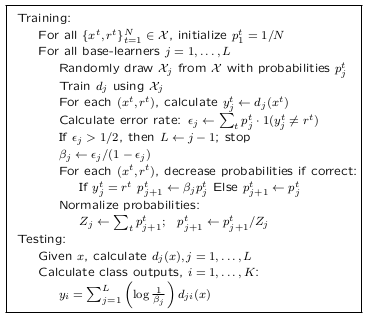
\includegraphics[width=14cm]{alg}


\end{description}
\section{Matrices Properties}
\begin{description}
    \item[Basic Matrix]
        $(\bA\bB)^T = \bB^T\bA^T$, 
    $(\bA\bB)^{-1} = \bB^{-1}\bA^{-1}$, $(\bA^T)^{-1} = (\bA^{-1})^T$, 
    $\mathbf{P}^{-1}+\bB^T \bR^{-1}\bB)^{-1}\bB^T\bR^{-1} = \mathbf{P}\bB^T(\bB
    \mathbf{P}\bB^T+\bR)^{-1}$, 
\item[Traces and Determinants] $Tr(\bA\bB) = Tr(\bB\bA)$, $Tr(\bA\bB\bC) = Tr(\bC\bB\bA) = Tr(\bB\bC\bA)$,
    $|\bA^{-1}| = \frac{1}{|\bA|}$, $\ba^T\bA\ba = Tr(\bA \ba\ba^T)$
\item[Matrix Derivatives] $\frac{\partial}{\partial \bx}(\bx^T\ba) =
    \frac{\partial}{\partial \bx}(\ba^T\bx) = \ba$,
    $\frac{\partial}{\partial\bx}(\bA\bB) = \frac{\partial \bA}{\partial \x}\bB
    +\bA\frac{\partial \bB}{\partial \bx}$, $\frac{\partial}{\partial
    x}(\bA^{-1}) = -\bA^{-1}\frac{\partial \bA}{\partial x}\bA^{-1}$, 
    $\frac{\partial}{\partial x}\ln |\bA| = Tr(\bA^{-1}\frac{\partial
    \bA}{\partial x})$, $\frac{\partial}{\partial A_{ij}}Tr(\bA\bB) = B_{ji}$,
    $\frac{\partial}{\partial \bA}Tr(\bA\bB) = \bB^T$, $\frac{\partial}{\partial
    \bA}Tr(\bA) = \mathbf{I}$, $\frac{\partial}{\partial \bA}Tr(\bA\bB\bA^T) =
    \bA(\bB+\bB^T)$, $\frac{\partial}{\partial \bA}\ln |\bA| = (\bA^{-1})^T$
\end{description}


\chapter{Convolutional Neural Networks}
\section{Motivation}
There exist a complex arrangement of cells within the visual cortex. These
cells are sensitive to small sub-regions of the input space, called a
\textbf{receptive field}, and are tiled in such a way as to cover the
entire visual field. These filters are local in input space and are thus
better suited to exploit the strong spatially local correlation present in
natural images.

Two basic cell types: Simple cells (S) and complex cells (C).
\begin{itemize}
    \item Simple Cells(S) respond maximally to specific edge-like stimulus
        patterns within their receptive field.
    \item Complex cells(C) have larger receptive fields and are locally
        invariant to the exact position of stimulus.
\end{itemize}

\section{Sparse Connectivity}
CNNs exploit spatially local correlation by \textbf{enforcing a local
connectivity pattern between neurons of adjacent layers}. 

Input hidden units in the $m$-th layer are connected to a local subset of
units in the $(m-1)$-th layer, which have spatially contiguous receptive
fields. 

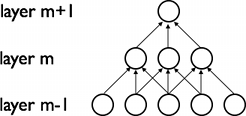
\includegraphics{sparse_1D_cnn}

\begin{itemize}
    \item Layer $m-1$ is the input retina. 
    \item Units in layer $m$ have receptive fields of width 3. Thus only
        connected to 3 adjacent neurons in the $(m-1)$-th layer.
    \item Layer $m$ have a similar connectivity with the layer below.
        $(m+1)$
\end{itemize}

We say that their receptive field with respect tot he layer below is 3,
but their receptive field with respect to the input is larger (it is 5).
The architecture thus confines the learnt ``filters'' to the spatially
local pattern.

\section{Shared Weights}
In CNNs, each sparse filter $h_i$ is additionally replicated across the
entire visual field. These ``replicated'' units form a \textbf{feature
map}, which share the same parameterization. (the receptive fields in the
same feature map share the same weight and bias for the sensitive region)

Gradient descent can still be used to learn such shared parameters, and
requires only a small change to the original algorithm. The gradient of a
shared weight is simply the sum of the gradients of the parameters being
shared.

Replicating units in this way allows for feature to be detected regardless
of their position in the visual field. Additionally, weight sharing offers
a very efficient way to do this, since it greatly reduces the number of
free parameter 

\section{Details and notation}
The $k$-th feature map at a given layer as $h^k$, whose filter with
weights $W^k$ and bias $b_k$, then the feature map $h^k$ is obtained as
follows (for $tanh$ non-linearities)
\[ h^k_{ij} = tanh\left( \left( W^k*x)_{ij} \right) + b_k \right)\]

To form a richer representation of the data, hidden layers are composed of
a set of multiple feature maps $\left\{ h^{(k)}, k = 0\dots K \right\}$

The weights of this layer can be parameterized as a 4D tensor (Tensors are
geometric objects that describe linear relations between vectors, scalars,
and other tensors. Elementary examples of such relations include the dot
product, the cross product and linear maps, vectors and scalars themselves
are also tensors.)
\begin{itemize}
    \item Destination feature map index
    \item Source feature map index
    \item Source vertical position index
    \item Source horizontal position index
\end{itemize}
\section{MaxPooling}
MaxPooling is a form of non-linear down-sampling. MaxPooling partitions
the input image into a set of non-overlapping rectangles and, for each
such sub-region, outputs the maximum value.

Useful for two reasons:
\begin{itemize}
    \item Reduces the computational complexity for upper layers
    \item Provides a form of translation invariance
\end{itemize}

Why it works: Imagine cascading a max-pooling layer with a convolutional
layer. There are $8$ directions in which one can translate the input image
into a single pixel. If max-pooling is done over a $2\times 2$ region, 
$3$ out of these $8$ possible configurations will produce exactly the same
output at the convolutional layer. For max-pooling over a $3\times 3$

\section{The Full Model: LeNet}
Graphical depiction: 

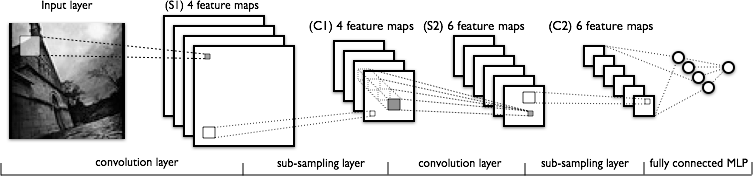
\includegraphics{mylenet}

The lower layers are composed to alternating convolution and max-mpooling
layers.

The upper layers however are fully-connected and correspond to a
traditional MLP


\chapter{Denoising Autoencoders}
An extension of a classical autoencoder and it was introduced as a
building block for deep networks. 
\section{Autoencoders}
An auto-encoder is trained to encode the input $\bx$ into some
representation $\mathbf{c}(\bx)$ so that the input can be reconstructed
from that representation. Hence the target output of the auto-encoder is
the auto-encoder input itself.

An autoencoder takes an input $ \bx\in [0,1]^d$

First maps it with an encoder to a hidden representation $\bf y \in [ 0,
1]^{d'}$ through a deterministic mapping:
\[ \by = s(\bW\bx + \mathbf{b}) \]
Where $s$ is a non-linearity such as the sigmoid. 

The latent representation $\bf y$, or \textbf{code} is then mapped back
(with a decorder ) into a \textbf{reconstruction} $\bf z$ of same shape as
$\bx$ though a similar transformation:
\[ \mathbf{z}= s(\bW' \by + \mathbf{b}')\].
Where $'$ does NOT indicate transpose, and $\mathbf{z}$ should be seen as
prediction of $\mathbf{x}$, given the code $\by$

The parameter of the model $W$ are optimized such that \textbf{the average
reconstruction error is minimized}. 

Measure the reconstruction error using the traditional squared error
$L(\bx, \mathbf{z}) = \|\bx - \mathbf{z}\|$

If the input is interpreted as either bit vectors or vectors of bit
probability by the reconstruction cross-entropy defined as (if $\bx|\by$
is in Gaussian):
\[ L_H(\bx, \mathbf{z}) = -\log P(\bx|\by) = -\sum_{k=1}^d\left[ \bx_k\log
\mathbf{z}_k + (1-\mathbf{x}_k)\log (1-\mathbf{z}_k)\right]\]

The hope: $\by$ is a distributed representation that captures the
coordinates along the main factors of variation in the data.

\section{Denoising Autoencoder}
The idea behind denoising autoencoders is that in order to force the
hidden layer to discover more robust features and prevent it from simply
learning the identity (copy the input to output), we train the autoencoder
to reconstruct the input from a corrupted version of it.

The denoising auto-encoder is a stochastic version of the auto encoder.
It does two things:
\begin{itemize}
    \item Try to encode the input (preserve the information)
    \item Try to undo the effect of a corruption process stochastically
        applied to the input of the auto-encoder.
\end{itemize}

The stochastic corruption process consists in randomly setting some of
the inputs (as many as half of them) to zero. Hence the denoising
auto-encoder is trying to \textbf{predict corrupted values from the
uncorrupted values}, for randomly selected subsets of missing patterns.
Note how being able to predict any subset of variables from the rest is a
sufficient condition for completely capturing the joint distribution
between a set of variables.

To convert the autodecoder class into a denoising autoencoder class, all
we need to do is to add a stochastic corruption step operating on the
input.



\chapter{Stacked Denoising Autoencoders(SDA)}
The denoising autoencoders can be stacked into form a deep network by
\textbf{feeding the latent representation(output code)} of the denoising
autoencoder found on the layer below as input to the current layer.

The unsupervised pre-training of such an architecture is done one layer at
a time. 

Each layer is trained as a denoising auto-encoder by minimizing
the reconstruction of its input (output code of the previous layer).

Once the first $k$-layers are trained, we can train the $(k+1)$-th layer
because we can now compute the code (latent representation) from the layer
below.

Once all layers are pre-trained, the network goes through a second stage
of training called \textbf{fine-tuning}.

\paragraph{Supervised fine-tuning} Minimize the prediction error on a
supervised task. 
\begin{enumerate}
    \item Add a logistic regression layer on top of the network (the out
        put code of the output layer)
    \item Train the entire network as we would train a multilayer
        perceptron. 
    \item At this point, we only consider the encoding parts of each
        auto-encoder.
\end{enumerate}

\chapter{Restricted Boltzmann Machines}
\section{Energy-Based Models (EBM)}
\begin{itemize}
    \item Associate a scalar energy to each configuration of the variables
    \item Learning: modify that energy so that its shape has desired
        properties.
\end{itemize}
Define a probability distribution through an energy function as follows:
\[
    p(x) = \frac{e^{-E(x)}}{Z}
\]
The normal factor $Z$ -- partition function

\[ Z = \sum_x e^{-E(x)}\]


An EBM can be learnt by performing stochastic gradient descent on the
empirical negative log-likelihood

As for logistic regression, log-likelihood:
\[ \mathcal{L}(\theta, \mathcal{D})  = \frac{1}{N} \sum_{x^{(i)}\in
\mathcal{D}}\log p(x^{(i)}\]
Loss function as being the negative log-likelihood:
\[ l(\theta, \mathcal{D}) = -\mathcal{L}(\theta, \mathcal{D})\]

Using the stochastic gradient: 
\[ - \frac{\partial \log p(x^{(i)}}{\partial \theta}\]
\subsection{EBMs with Hidden Units}
Consider an observed part $x$ and a hidden part $h$:
\[ P(x) = \sum_h P(x,h) = \sum_h \frac{e^{-E(x,h)}}{Z}\]

\textbf{Free Energy}
\[ \mathcal{F}(x) = -\log\sum_h e^{-E(x,h)}\]
Then
\[ P(x) = \frac{e^{-\mathcal{F}(x)}}{Z}
\]
with $Z = \sum_x e^{-\mathcal{F}(x)}$

Negative log-likelihood gradient:
\[ -\frac{\partial \log{p(x)}}{\partial \theta} = \frac{\partial
    \mathcal{F}(x)}{\partial \theta} -
    \sum_{\hat{x}}p(\hat{x})\frac{\partial\mathcal{F}(\hat{x})}{\partial
    \theta}
\]

The positive and negative phase reflect their effect on the probability of
training data.

It is usually difficult to determine this gradient analytically, as it
involves the computation of $E_p\left[ \frac{\partial
\mathcal{F}(x)}{\partial \theta} \right]$, an expectation over all
possible configuration of the input $x$.

Making this computation tractable is to \textbf{estimate the expectation} using a
fixed number of model samples.
\begin{itemize}
    \item Samples used to estimate the negative phase gradient are
        referred to as negative particles, denoted as $\mathcal{N}$
    \item The gradient can be written as:
        \[ 
            -\frac{\partial\log{p(x)}}{\partial \theta}\approx
            \frac{\partial \mathcal{F}(x)}{\partial \theta} -
            \frac{1}{|\mathcal{N}|}\sum_{\hat{x}\in\mathcal{N}}\frac{\partial
                \mathcal{F}(\hat{x})}{\partial \theta}
            \]
\end{itemize}

\section{Restricted Boltzmann Machines (RBM)}
A particular form of log-linear Markov Random Field, for which the
\textbf{energy function is linear} in its free parameters.

Two-layer network, in which stochastic, binary \emph{feature detectors}
using weighted connections.

\begin{itemize}
    \item The pixels correspond to visible units
    \item The feature detectors correspond to hidden units
\end{itemize}

Assume that the hidden and visible variables are binary.

\begin{enumerate}
    \item \textbf{Energy} Joint Configuration $(\mathbf{v}, \mathbf{h})$  (visible and
        hidden)
        \[ E(\mathbf{v,h}) = -\sum_{i\in visible}a_i v_i - \sum_{j\in hidden}b_j
        h_j - \sum_{i,j}v_ih_jw_{ij}\]
        $a_i$ and $b_j$ are bias and $w_{ij}$ is the weight
    \item  Probability to every pair of a visible and a hidden vector:
        \[ p(\bv) = \sum_{\bh} p(\bv, \bh) = \frac{1}{Z}\sum_{\bh} e^{-E(\bv,
        \bh)}\]
        Z is given by:
        \[ Z = \sum_{\bv, \bh} e^{-E(\bv,\bh)}\]
    \item Network assigns to a visible vector $\mathbf{v}$:
        \[
            p(\bv) = \frac{1}{Z}\sum_{\bh} e^{-E(\bv, \bh)}
        \]
    \item Raise the probability of the network assigns a training image:
        lower the energy of that image and raise the energy of other images
        \verb|=>| By adjusting the weights and biases.
    \item Derivative of the log probability:
        \[\frac{\partial \log{p(\bv})}{\partial w_{ij}} = \langle
        v_ih_j\rangle_{data} - \langle v_i h_j\rangle_{model}\]
        Angle brackets denote expectations under the distribution specified by the
        subscript that follows
    \item 
        The learning rule:
        \[ \Delta w_{ij} = \epsilon(\langle
            v_ih_j\rangle_{data} - \langle v_i h_j\rangle_{model})
        \]
        Where $\epsilon$ is the learning rate.
    \item Ease to get a unbiased sample of $\langle v_ih_j \rangle$
        \begin{equation*}
            p(h_j = 1|\bv)  =  \sigma(b_j + \sum_i v_i w_{ij} \\
            p(v_i = 1|\bh)  =  \sigma(a_i + \sum_j h_j w_{ij}
        \end{equation*}
\end{enumerate}



Energy function:
\[ E(v, h) = -b'v - c'h - h'Wv\]
$W$ -- The weights connecting hidden and visible units and \\
$b$, $c$ -- the offsets of the visible and hidden layers respectively.

Free energy formula:
\[ 
    \mathcal{F}(v) = -b'v - \sum_i \log \sum_{h_i} e^{h_i(c_i+W_i v)}
\]

Visible and hidden units are conditionally independent given one-another:
\begin{equation*}
    p(h|v) = \prod_{i}p(h_i|v) \\
    p(v|h) = \prod_j p(v_j|h)
\end{equation*}

\subsection{Binary Units}
In the case of binary units $v_j, h_i \in \left\{ 0, 1 \right\}$:
\begin{equation*}
    P(h_i = 1| v) = sigm(c_i + W_i v)\\
    P(v_j = 1|h) = sigm(b_j + W'_j h)
\end{equation*}
Free energy can be simplifies to:
\[ \mathcal{F}(v) = - b'v - \sum_i \log(1 + e^{c_i + W_j v)}\]

\section{Contrastive divergence multi-layer RBMs}
\subsection{Boltzmann machines}
$X$ observed and $H$ hidden. Their joint given by Boltzmann distribution
associate with energy:
\[ P(X = x, H= h) = \frac{\exp{[-E(x,h)]}}{Z} \]
$Z$ is the appropriate normalization constant:
\[ Z = \sum_{x,h}\exp{(-E(x,h))}\]

Energy function is a quadratic polynomial, $z=(x,h)$
\[ E(z) = -\sum_i b_i z_i - \sum_{ij}w_{ij}z_i z_j\]
$z_i \in {0, 1}$

If $X = x$ observed, $H$ remains hidden, the likelihood involves a sum
over all configurations of $H$:
\[ P(X = x) = \sum_h P(X = x, H = h) = \sum_h
    \frac{\exp{(-E(x,y))}}{Z}
\]

Summing over $h$ and $x$ (in denominator $Z$) are both
intractable.

Restricted Boltzmann Machine: interactions between hidden units are
removed, so the sum over $h$ becomes tractable.

Derivatives(non-tractable):
\begin{eqnarray*}
    \frac{\partial -\log P(x)}{\partial \theta} &=&
    \frac{\partial -\log \sum_h \frac{\exp (-E)}{Z}}{\partial \theta} \\
    &=&\frac{\partial \left\{ -\log[\sum_h\exp (-E)]+\log Z
    \right\}}{\partial \theta} \\
    &=& \sum_h \frac{exp(-E)}{\sum_h \exp(-E)} \cdot
    \frac{\partial E}{\partial \theta} - \frac{1}{Z}\sum_{x,h} \exp\left[
    -E(x,h) \right]\frac{\partial E}{\partial \theta} \\
    &=&\sum_h \left[ \frac{\exp(-E)}{\sum_h
    \exp(-E)}\frac{\partial E}{\partial H}\right] \frac{\partial
    E}{\partial \theta} - \sum_{x,h} \frac{\exp[-E(x,h)]}{Z}\frac{\partial
    E}{\partial \theta} \\
 &=& \sum_h P(H=h|X=x)
    \frac{\partial E(h,x)}{\partial \theta} \mbox{ [this is the POSITIVE
    phase contribution] }\\  & &- \sum_{h,x}  P(H=h,X=x) \frac{\partial
    E(h,x)}{\partial \theta} \mbox{ [this is the NEGATIVE phase
    contribution] } 
\end{eqnarray*}

The standard way to estimate the gradient, is to avoid perform an MCMC
scheme to obtain one or more samples from $P(h|x)$
scheme
\subsection{Restricted Boltzmann Machines}
If we set the weight between $h_i$ and $h_j$ and the weight between $x_i$
and $x_j$ we obtain a RBM.

All the $H_i$'s become independent when conditioning on X, and all the
$X_i$ become independent when conditioning on $H$.

\subsection{Energy functions for RBM}
Note that $w_{ij} = w_{ji}$

Energy term for binomial unit $i$ with value $v_i$ and inputs
    $u_j$.
    \[
        E(v_i, u_j) = -b_i v_i - \sum_j w_{ij} v_i u_j 
    \]
    \[ ==> P(v_i=1 | u) = \frac{exp(b_i + \sum_j w_{ij} u_j) }{ 1 +
    exp(b_i + \sum_j w_{ij} u_j) } = sigmoid\left(b_i + \sum_j w_{ij}
    u_j\right) \]

Energy term for fixed-variance Gaussian unit $i$ with value
    $v_i$ and inputs $u_i$:
    \[ a_i^2 v_i^2 - b_i v_i - \sum_j w_{ij} v_i u_j\]
    \[ P(y|x) = \frac{\exp(-E(x,y)) }{ \sum_y \exp(-E(x,y)) } \]

\subsection{Update Rule}
Use $Z = \sum_{x,y} \exp[-E(x,y)]$:
\[P(x,y) = \frac{\exp[-E(x,y)]}{Z} \]

For any energy-based Boltzmann distribution:
\begin{eqnarray*}
      \frac{\partial}{\partial \theta}(-\log P(x) ) &=&
    \frac{\partial}{\partial \theta} \left(- \log \sum_y P(x,y)\right) \\
     &=& \frac{\partial}{\partial \theta}\left(- \log
    \sum_y \frac{\exp(-E(x,y))}{Z}\right) \\
    &=&  - \frac{Z}{\sum_y \exp[-E(x,y)]}
    \left( \sum_y \frac{1}{Z} \frac{\partial \exp[-E(x,y)]}{\partial
    \theta} - \sum_y \frac{\exp[-E(x,y)]}{Z^2} \frac{\partial Z}{\partial
    \theta}\right) \\
    &=&  \sum_y
    \left(\frac{\exp[-E(x,y)]}{\sum_{\hat y} \exp[-E(x,\hat y)]}
    \frac{\partial E(x,y)}{\partial \theta}\right) + \frac{1}{Z}
    \frac{\partial Z}{\partial \theta} \\
    &=& \sum_y P(y|x) \frac{\partial E(x,y)}{\partial \theta} -
    \frac{1}{Z} \sum_{x,y} \exp[-E(x,y)] \frac{\partial
    E(x,y)}{\partial \theta} \\
    &=& \sum_y P(y|x) \frac{\partial
    E(x,y)}{\partial \theta} - \sum_{x,y} P(x,y) \frac{\partial
    E(x,y)}{\partial \theta} \\
    &=& \mathbb{E}\left[\left. \frac{\partial
    E(x,y)}{\partial \theta} \right| x \right] - \mathbb{E}\left[ \frac{\partial
    E(x,y)}{\partial \theta} \right] 
    &=& \mbox{positive phase contribution} - \mbox{negative phase
    contribution}
\end{eqnarray*}

\[ \sum_y P(y|x) \frac{\partial E(x,y)}{\partial \theta_i} =
\sum_{y_i}P(y_i|x) \frac{\partial E_i(x,y_i)}{\partial \theta_i}\]
with $\theta$ the parameters associated with $y_i$

\subsubsection{Sampling in an RBM}
Samples of $p(x)$ can be obtained by running a Markov chain to convergence,
using Gibbs sampling as the transition operator.

Gibbs sampling of the joint of $N$ variables $S = (S_1, \dots, S_N)$ si
done through a sequence of $N$ sampling substeps of the form $S_i \sim
p(S_i|S_{-i})$ where $S_{-i}$ contains the $N-1$ other random variable in
the $S$ excluding $S_i$.

For RBM:
\begin{itemize}
    \item $S$ consists of visible and hidden units.
    \item Since they are conditionally independent, one can perform block
        Gibbs sampling. In this setting, visible units are sampled
        simultaneously given fixed values of hidden units.
     \item Markov Chain:
         \begin{eqnarray*}
             h^{(n+1)} &\sim & sigm(W' v^{(n)} + c) \\
             v^{(n+1)} & \sim & sigm(W h^{(n+1)} + b)
         \end{eqnarray*}
         $h^{(n)}$ refers to the set of all hidden units at the n-th step
         of the Markov chain.

         What it means: $h_i^{(n+1)}$ is chosen to be $1$ with probability
         $sigm(W_i' v^{(n)} + c_i)$ and $v_j^{(n+1}$ is chosen to be $1$
         with probability
         $sigm(W_{\cdot j}h^{(n+1)} + b_j$

         As $t \rightarrow \infty$ samples $(v^{(t)}, h^{(t)})$ are
         guaranteed to be accurate samples of $p(v,h)$.

\end{itemize}


\end{document}
